\documentclass{tufte-handout}

\usepackage{amsmath}
\usepackage{amsfonts}
\usepackage{booktabs}
\usepackage{upquote}
\usepackage{multicol}
\usepackage{units}    % non-stacked fractions and better unit spacing
\usepackage{IEEEtrantools}
\usepackage{subcaption}

\usepackage{listings}
\lstset{
    breaklines,
    basicstyle=\ttfamily\small,
}



\usepackage{graphicx}
\setkeys{Gin}{width=\linewidth,totalheight=\textheight,keepaspectratio}
\graphicspath{{graphics/}}

\title{Assignment for DAT246\slash DIT246}
\author[Carl Holmberg]{Carl Holmberg}
%\date{}


\begin{document}

\maketitle

\begin{abstract}
    \noindent Abstract
\end{abstract}

%\printclassoptions

% Introduction
\newthought{This report will} detail the process of investigating wheter the new technology is better than the old technology.

\subsection*{General notes}
There are two different ways i am thinking about going about this.
One method is using a \textit{GLM} and another is using the treament analysis in the book.


\subsection{Data}
% \textit{Description of the data, i.e., descriptive statistics, if there is a need to standardize\slash normalize, etc.}
\newthought{The data constists} of 70 individual subjects that participated in an experiment with a $2 \times 2$ design.


From the data, four different cases were picked, the combinations of old \slash new technology and more \slash less experience.
A simple table of descriptive statistics containing these cases was created and a density plot for each of the cases.
The result of this analysis can be shown in figure \ref{fig:ds}


\begin{figure}[h]
    \begin{subtable}[t]{0.52\textwidth}
        \caption{Descriptive Statistics}
        \resizebox{\textwidth}{!}{
            \begin{tabular}{cccc}
                technique & experience & mean     & sd       \\ \hline
                OT        & LE         & 5.282609 & 2.428196 \\
                OT        & ME         & 4.708333 & 1.731528 \\
                NT        & LE         & 4.555556 & 1.816034 \\
                NT        & ME         & 4.250000 & 1.700384
            \end{tabular}
        }
    \end{subtable}
    \begin{subfigure}[t]{0.43\textwidth}
        \caption{Density Chart}
        \centering
        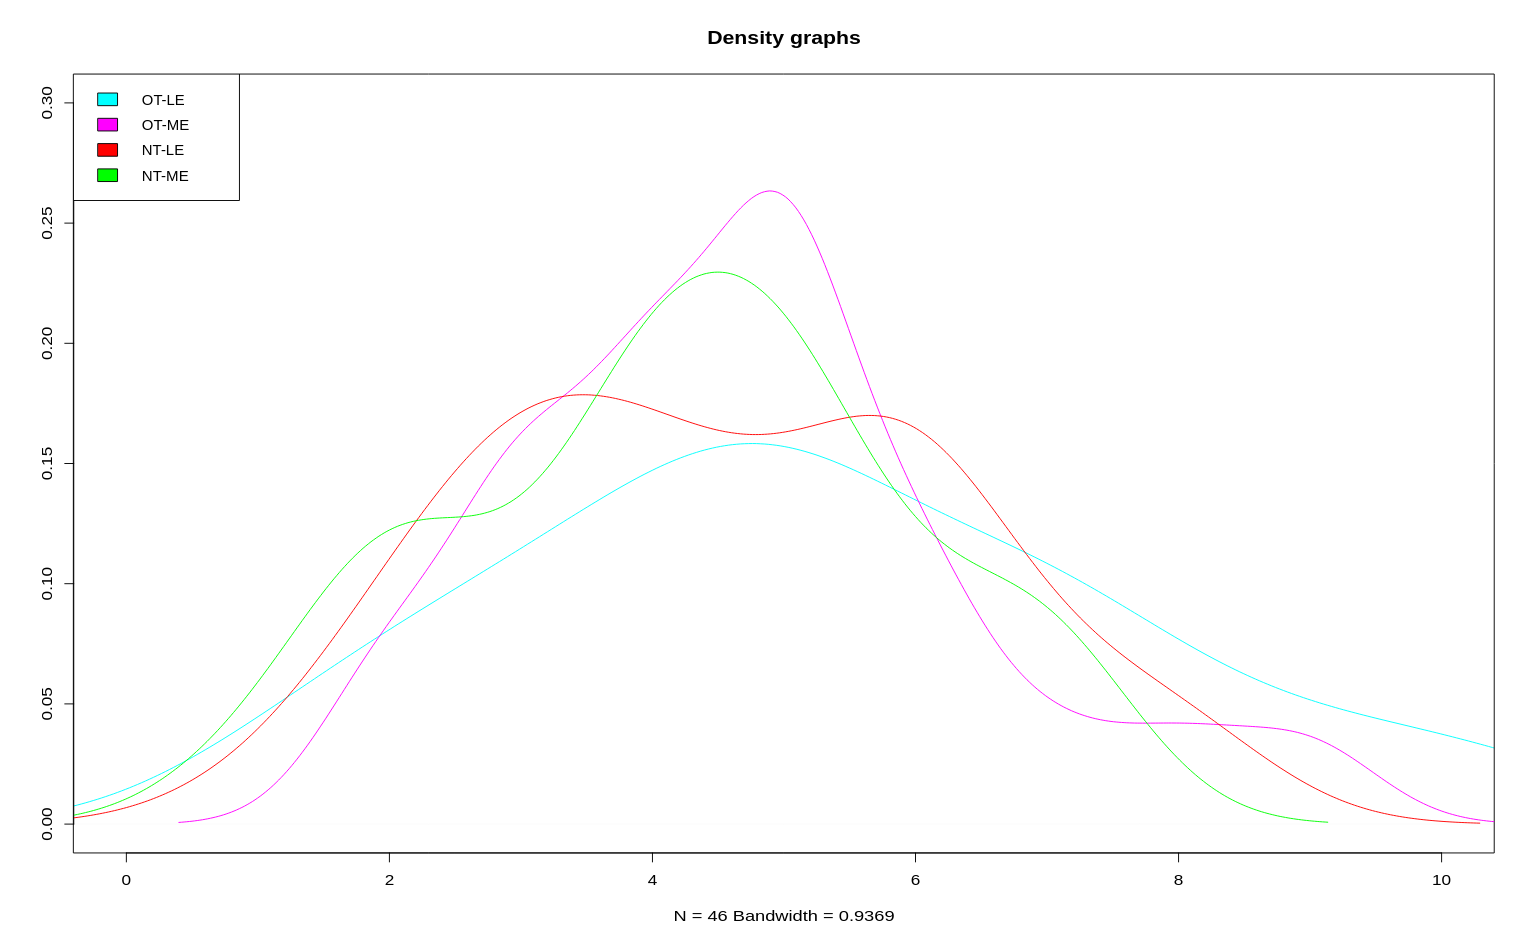
\includegraphics[width=\textwidth]{density-chart.png}
    \end{subfigure}
    \caption{Figure showing both the descriptive statistics of the four cases and a colorized plot containing the densities.}
    \label{fig:ds}
\end{figure}

\newthought{The table and plot} shows us that the difference when looking at the data in this way shows much similarity between the techniques.

Two methods will be used.
The first method will use a \textit{GLM}


\subsection{Defense of likelihood}
% \textit{A defense of your likelihood(s). We assume you will develop at least two models with, perhaps, different likelihoods. Please use the same math notation to describe your model(s) as they do in the course book, e.g.,\cite{mcelreath20SR}
%     {\footnotesize
%         \begin{IEEEeqnarray*}{rCl}
%             \mathrm{L}_i & \sim & \mathrm{Binomial}(n_i,p_i)\\
%             \mathrm{logit}(p_i) & = & \alpha_{\mathrm{SUBJECT}[i]} + (\beta_P + \beta_{PC}C_i)P_i\\
%             \alpha_{\mathrm{SUBJECT}} & \sim & \mathrm{Normal}(0,10) \\
%             \beta_P & \sim & \mathrm{Normal}(0,10)\\
%             \beta_{PC} & \sim & \mathrm{Normal}(0,10)
%         \end{IEEEeqnarray*}
%     }}



\subsection{Final priors}
\textit{A discussion regarding the priors you have chosen for your `final' model. Defend them and show what happens if you change priors!}-

\subsection{Final results and comparisons}
\textit{Results from running your `final' model with \texttt{ulam()}, comparing it with other model(s) using WAIC or LOO,\footnote{The \textsf{rethinking} package has a \texttt{compare()} function for this} and reason about what the results means.}

\subsection{DAG}
\textit{Adding a DAG is always nice (use the \texttt{ggdag} package in \textsf{R}). If you can explain direct and indirect causal effects without one then sure.\footnote{\url{https://ggdag.malco.io}}}

\subsection{Diagnostics}
\textit{Presentation of diagnostics from running \textsf{Stan} on the `final' model, e.g., caterpillar traces (or trankplots),\footnote{\url{http://mc-stan.org/assets/img/bayesplot/mcmc_trace-rstan.png}} $\hat{R}$ values, and\slash or effective sample size. There's no reason to show traceplots that take up a page!}

\subsection{Interpretation}
\textit{Interpretation of what the results mean from a practical point of view, i.e, which technique is better, does experience influence the results, and how does the analysis support your argument?}


\nobibliography{sample-handout}
\bibliographystyle{abbrvnat}

\end{document}